\section{Updating the Model}\label{model-update}
This section describes an algorithm for reliable model updates.
For convex loss minimization, Stochastic Gradient Descent converges to an optimum from any initialization as long each gradient descent step is unbiased.
We show how we can leverage this property to prove convergence for interactive data cleaning regardless of the inaccuracy of the initial model--as long as the analyst does not systematically exclude certain data from cleaning. 
%To do so, we will sample yet-to-be-cleaned data in batches, where every record has a non-zero probability $p(i)$ of being sampled.
%Sections \ref{dist-samp} show how to select a non-uniform $p(\cdot)$ and the analysis in this section applies for any sampling distribution $p(\cdot) > 0$.
The updater only assumes that it is given a sample of data $S_{dirty}$ from $R_{dirty}$ where $i \in S_{dirty}$ has a known sampling probability $p(i)$.

\subsection{Geometric Derivation}\label{geod}
The update algorithm intuitively follows from the convex geometry of the problem.
Consider the problem in one dimension (i.e., the parameter $\theta$ is a scalar value), so then the goal is to find the minimum point ($\theta$) of a curve $l(\theta)$.
The consequence of dirty data is that the wrong loss function is optimized.
Figure \ref{update-arch2}A illustrates the consequence of the optimization.
The red dotted line shows the loss function on the dirty data.
Optimizing the loss function finds $\theta^{(d)}$ that at the minimum point (red star).
However, the true loss function (w.r.t to the clean data) is in blue, thus
the optimal value on the dirty data is in fact a suboptimal point on clean curve (red circle).

\begin{figure}[ht!]
\centering
 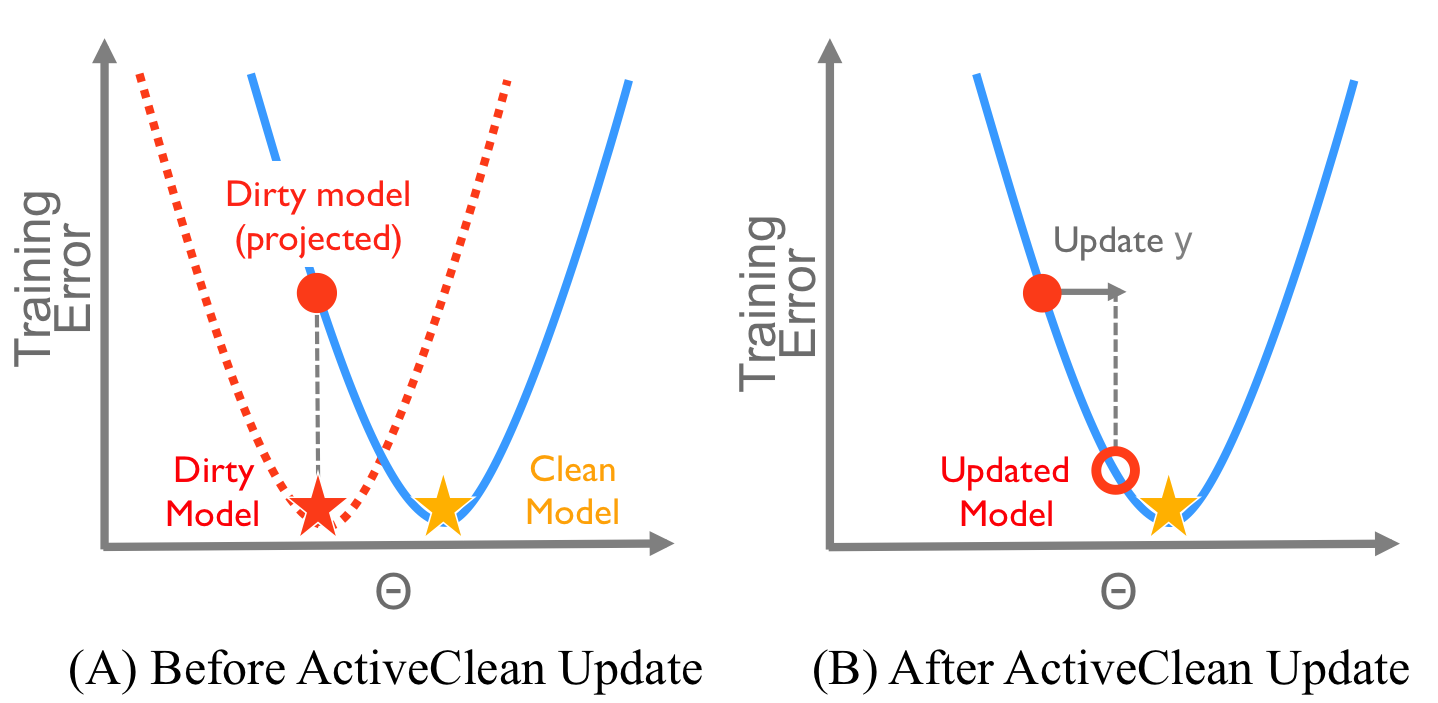
\includegraphics[width=\columnwidth]{figs/update-arch2.png}\vspace{-1em}
 \caption{(A) A model trained on dirty data can be thought of as a sub-optimal point w.r.t to the clean data. (B) The gradient gives us the direction to move the suboptimal model to approach the true optimum. \label{update-arch2}}\vspace{-1em}
\end{figure}

The optimal clean model $\theta^{(c)}$ is visualized as a yellow star.
The first question is which direction to update $\theta^{(d)}$ (i.e., left or right).
For this class of models, given a suboptimal point, the direction to 
the global optimum is the gradient of the loss function.
The gradient is a $p$-dimensional vector function of the current model $\theta^{(d)}$ and the clean data.
Therefore, \sys needs to update $\theta^{(d)}$ some distance $\gamma$ (Figure \ref{update-arch2}B):
\[
\theta^{new} \leftarrow \theta^{(d)} - \gamma \cdot \nabla\phi(\theta^{(d)})
\]
At the optimal point, the magnitude of the gradient will be zero.
So intuitively, this approach iteratively moves the model downhill (transparent red circle) -- correcting the dirty model until the desired accuracy is reached.
However, the gradient depends on all of the clean data, which is not available, and \sys will have to approximate the gradient from a sample of newly cleaned data.
%The main intuition is that if the gradient steps are on average correct, the model still moves downhill albeit with a reduced convergence rate proportional to the inaccuracy of the sample-based estimate.

To derive a sample-based update rule, the most important property is that sums commute with derivatives and gradients.
The convex loss class of models are sums of losses, so given the current best model $\theta$, the true gradient $g^*(\theta)$ is:
\[
g^*(\theta) = \nabla\phi(\theta) = \frac{1}{N} \sum_{i=1}^N \nabla\phi(x_i^{(c)},y_i^{(c)},\theta)
\]
\sys needs to estimate $g^*(\theta)$ from a sample $S$, which is drawn from the dirty data $R_{dirty}$.
 Therefore, the sum has two components which are the gradient from the already clean data $g_C$ and $g_S$ a gradient estimate from a sample of dirty data to be cleaned:
\begin{equation}
g(\theta) = \frac{\mid R_{clean} \mid}{\mid R \mid} \cdot g_C(\theta) + \frac{\mid R_{dirty} \mid}{\mid R \mid} \cdot g_S(\theta)\label{unbia}
\end{equation}
$g_C$ can be calculated by applying the gradient to all of the already cleaned records:
\[
g_C(\theta) = \frac{1}{\mid R_{clean}\mid}\sum_{i \in R_{clean}}\nabla\phi(x_i^{(c)},y_i^{(c)},\theta)
\] 
$g_S$ can be estimated from a sample by taking the gradient w.r.t each record, and re-weighting the average by their respective sampling probabilities.
Before taking the gradient the cleaning function $C(\cdot)$ is applied to each sampled record.
Therefore, let $S$ be a sample of data, where each $i \in S$ is drawn with probability $p(i)$:
\[
g_{S}(\theta) = \frac{1}{\mid S \mid} \sum_{i \in S}\frac{1}{p(i)}\nabla\phi(x_i^{(c)},y_i^{(c)},\theta)
\]
Then, at each iteration $t$, the update becomes:
\[
\theta^{(t+1)} \leftarrow \theta^{(t)} - \gamma \cdot g(\theta^{(t)})
\]

\subsection{Model Update Algorithm}\label{update-alg}
We present pseudocode for one iteration of the update algorithm.
To summarize, the algorithm is initialized with $\theta^{(0)} = \theta^{(d)}$ which is the dirty model.
There are three user set parameters the budget $k$, batch size $b$, and the step size $\gamma$.
In the following section, we will provide references from the convex optimization literature that allow the user to appropriately select these values.
At each iteration $t=\{1,...,T\}$, the cleaning is applied to a batch of data $b$ selected from the set of candidate dirty records $R_{dirty}$.
Then, an average gradient is estimated from the cleaned batch and the model is updated.
Iterations continue until $k = T \cdot b$ records are cleaned.

\begin{enumerate}[noitemsep]
	\item Take a sample of data $S$ from $R_{dirty}$ 
	\item Calculate the gradient over the sample of newly clean data and call the result $g_S(\theta^{(t)})$
	\item Calculate the average gradient over all of the already clean records in $R_{clean}=R-R_{dirty}$, and call the result $g_C(\theta^{(t)})$
	\item Apply the following update rule, which is a weighted average of the gradient on the already clean records and newly cleaned records:
	\[
	\theta^{(t+1)} \leftarrow \theta^{(t)} - \gamma \cdot(\frac{\mid R_{dirty} \mid}{\mid R \mid} \cdot g_S(\theta^{(t)}) + \frac{\mid R_{clean} \mid}{\mid R \mid} \cdot  g_C(\theta^{(t)}))
	\]
	\item Append the newly cleaned records to set of previously clean records $R_{clean} = R_{clean} \cup S$ 
\end{enumerate} 

This basic algorithm will serve as the scaffolding for the optimizations in the subsequent sections.
For example, if we know a record is likely to be clean, we can move it from $R_{dirty}$ to $R_{clean}$ without having to sample it.
Similarly, we can set the sampling probabilities $p(\cdot)$ to favor records that are likely to affect the model.

\subsection{Analysis with Stochastic Gradient Descent}\label{sgd}
The update algorithm can be formalized as a class of very well studied algorithms called Mini-batch Stochastic Gradient Descent (SGD).
In SGD, random subsets of data are selected at each iteration and the average gradient is computed for every batch.
The basic condition for convergence is that the gradient steps need to be on average correct.
We provided the intuition that this is the case in Equation \ref{unbia}, and this can be more rigorously formalized as an unbiased estimate of the true gradient~(see T.R \cite{activecleanarxiv}).
Then model is guaranteed to converge essentially with a rate proportional to the inaccuracy of the sample-based estimate.

One key difference with the SGD models applied in model training frameworks is that \sys applies a \emph{full} gradient step on the already clean data and averages it with a stochastic gradient step (i.e., calculated from a sample) on the dirty data. 
This is because that data is already clean and we assume that the time-consuming step in the data cleaning and not the numerical operations.
The update algorithm can be thought of as a variant of SGD that lazily materializes the clean value.
As data is sampled at each iteration, data is cleaned when needed.
It is well known that even for an arbitrary initialization SGD makes significant progress in less than one epoch (a pass through the entire dataset) \cite{bottou2012stochastic}.
However, the dirty model can be much more accurate than an arbitrary initialization.

\vspace{0.25em}

\noindent\textbf{ Setting the step size $\gamma$: } There is extensive literature in machine learning for choosing the step size $\gamma$ appropriately. $\gamma$ can be set either to be a constant or decayed over time. Many machine learning frameworks (e.g., MLLib, Sci-kit Learn, Vowpal Wabbit) automatically set this value. 
In the experiments, we use a technique called inverse scaling where there is a parameter $\gamma_0=0.1$, and at each iteration it decays to $\gamma_t = \frac{\gamma_0}{\mid S \mid t}$. 

\vspace{0.25em}

\noindent\textbf{ Setting the batch size $b$: } The batch size should be set by the user to have the desired properties.
Larger batches will take longer to clean and will make more progress towards the clean model but will have less frequent model updates.
On the other hand, smaller batches are cleaned faster and have more frequent model updates.
In the experiments, we use a batch size of 50 which converges fast but allows for frequent model updates.
If a data cleaning technique requires a larger batch size than 50, \sys can abstract this size away from the update algorithm and apply the updates in smaller batches.
For example, the batch size set by the user might be $b=1000$, but the model updates after every $50$ records are cleaned.
We can disassociate the batching requirements of SGD and the batching requirements of the data cleaning technique.

\vspace{0.25em}

\noindent\textbf{Convergence Conditions and Properties}
The convergence rates of SGD are also well analyzed \cite{dekel2012optimal,bertsekas2011incremental,zhao2014stochastic}. 
The analysis gives a bound on the error of intermediate models and the expected number of steps before achieving a model within a certain error. 
For a general convex loss, a batch size $b$, and $T$ iterations, the convergence rate is bounded by $O(\frac{\sigma^2}{\sqrt{bT}})$. 
$\sigma^2$ is a measure of how well the sample gradient estimates the gradient over the entire dataset, and $\sqrt{T}$ shows that each iteration has diminishing returns.
$\sigma^2$ is the variance in the estimate of the gradient at each iteration:
\[
\sigma^2 = \mathbb{E}(\|g - g^*\|^2)
\]
where $g^*$ is the gradient computed over the full data if it were fully cleaned.
This property of SGD allows us to bound the model error with a monotonically decreasing function of the number of records cleaned, thus satisfying the reliability condition in the problem statement.

Gradient descent techniques still apply to non-convex losses as they are widely applied in graphical model inference and deep learning. Instead of converging to a global optimum
they converge to a locally optimal value. However, there is a dependence on the initialization.
ActiveClean will converge to the closest locally optimal value to
the dirty model (which is how we initialize). Because of this, it is harder to reason about
the objective quality of the results and to define accuracy.
 Different initializations will lead to different local
optima, and thus, introduces a complex dependence on the
initialization with the dirty model.

\begin{example}\label{upex}
Recall that the analyst has a dirty SVM model on the dirty data $\theta^{(d)}$.
She decides that she has a budget of cleaning $100$ records, and decides to clean the 100 records in batches of 10 (set based on how fast she can clean the data, and how often she wants to see an updated result).
All of the data is initially treated as dirty with $R_{dirty} = R$ and $R_{clean} = \emptyset$.
The gradient of a basic SVM is given by the following function:
\[
\nabla\phi(x,y,\theta) =
\begin{cases}      
-y\cdot\boldsymbol{x} ~~~~~~ \text{ if } y\boldsymbol{x}\cdot\theta < 1 \\
~~~~~~~0\ ~~~~~~\text{ if } y\boldsymbol{x}\cdot\theta \geq 1      
\end{cases}
\]

For each iteration $t$, a sample of 10 records $S$ is drawn from $R_{dirty}$.
\sys then applies the cleaning function to the sample.
Using these values, \sys estimates the gradient on the newly cleaned data:
\[
\frac{1}{10} \sum_{i \in S}\frac{1}{p(i)}\nabla\phi(x_i^{(c)},y_i^{(c)},\theta)
\]
\sys also applies the gradient to the already clean data (initially non-existent):
\[
\frac{1}{\mid R_{clean}\mid}\sum_{i \in R_{clean}}\nabla\phi(x_i^{(c)},y_i^{(c)},\theta)
\]
Then, it calculates the update rule:
\[
	\theta^{(t+1)} \leftarrow \theta^{(t)} - \gamma \cdot(\frac{\mid R_{dirty} \mid}{\mid R \mid} \cdot g_S(\theta^{(t)}) + \frac{\mid R_{clean} \mid}{\mid R \mid} \cdot  g_C(\theta^{(t)}))
\] 
Finally, $R_{dirty} \leftarrow R_{dirty} - S$, $R_{clean} \leftarrow R_{clean} + S$, and continue to the next iteration.
\end{example}
